% ============================================================================
\section{Results}
\label{sec:results}
% ============================================================================
Table~\ref{tab:verdicts} gives the verdict on every preregistered hypothesis; the subsections that follow report the evidence in the order of the four properties.

\begin{table*}[!t]
\caption{Hypotheses and verdicts. $^{\mathrm{a}}$Rests on the amendment written after early results.}
\label{tab:verdicts}
\centering\footnotesize
\setlength{\tabcolsep}{4pt}
\begin{tabularx}{\textwidth}{@{}P{5.2cm} L P{3.9cm}@{}}
\toprule
Hypothesis & Result & Verdict \\
\midrule
Invariants A1 and A3$_\omega$ & no violation & met \\
H1: lower bound of RA $\geq 0.70$ & 16/16 (lower bound 0.829); 15/16 (0.736) counting only the first attempt; 8/16 (0.279) without aligning the rounding convention of the examples & accepted, conditional on the rounding convention \\
H2a: upper bound of SER $\leq 0.25$ & SER 3/18, upper bound 0.377 & not accepted \\
H2b: CAR of the pipeline above B3 and B4 & 8/18 against 8/18 and 9/18; McNemar $p = 0.75$ and $p = 1.0$; Holm-adjusted $p = 1$ & not accepted \\
H2b: SER not worse by more than 0.10 & against B3, difference $-0.222$ with upper bound 0.004; against B4, difference 0 with upper bound 0.153 & met against B3, not against B4 \\
H3a: lower bound of OAR $\geq 0.75$ & transplanted chain 31/33 (0.821), mostly through masking; regenerated chain$^{\mathrm{a}}$ 23/33 (0.540) & accepted in the registered analysis, not robust \\
H3b: triggered errors within the noise bound & 29 cases on the regenerated chain$^{\mathrm{a}}$ against a noise bound of 0 & not supported \\
H4a: lower bound of recall $\geq 0.70$ & recall 0.91, cluster CI 0.75--1.00 & accepted \\
H4b: $F_2$ of the detector above B5(i) and B5(ii) & $+0.193$ (CI 0.062--0.400) against B5(ii); $-0.006$ (CI $-0.110$ to 0.058) against B5(i) & not accepted \\
\bottomrule
\end{tabularx}
\end{table*}

\subsection{Instrument Validity}
\label{sec:res-instruments}
The gold knowledge base agreed with the independent calculation on all 50 GT3 cases and all 2,107 of their observations. Its remaining differences from the other references are one-rupiah rounding and errors in the official examples. The others come from a labor-agreement clause that the knowledge base does not formalize and from examples dated before an agreement took effect (Table~\ref{tab:refs} in Appendix~\ref{app:tables}). The DJP calculator matched 15 of 20 monthly cases and all 90 final-period rows; on the other five monthly cases it differed by Rp1, because it truncates fractions where the knowledge base rounds. The development examples of GT1 matched on 22 of 26 cases, and the 13 material differences are errors in the official examples.

One of the official examples shows why adjudication is needed. The example in PMK 10/2025 caps the occupational expense of an employee who works part of the year month by month, at Rp4,550,000. The examples in PMK 168/2023 and PMK 105/2025 apply an annual cap of Rp4,750,000 to the same situation, and the knowledge base follows them. The GT1 holdout first matched 6 of 10 cases and 221 of 235 observations and exposed two errors in the gold knowledge base. It matched 8 of 10 cases and 232 of 235 observations after the correction, and its two remaining material differences concern how pension contributions were mapped. Adding 17 targeted cases raised the mutation score over nonequivalent mutants from 0.90 to 1.00. The second reader agreed on the values of 90\% of the gold units, with a Krippendorff's $\alpha$ of 0.79 for the start dates of added elements and 0.61 over all units.

\subsection{Expressiveness of the Representation}
\label{sec:res-expressiveness}
All 16 unseen changes were expressed as updates without changing the engine, and their 100 examples with 2,609 values were reproduced exactly (RA 16/16, CI 0.794--1.000, one-sided lower bound 0.829). Fifteen changes succeeded at the first attempt. The result depends on one convention update, because the examples round withholding down, like the DJP calculator, whereas the knowledge base rounds to the nearest rupiah under PER-11/PJ/2025. Eight of the 16 changes pass without that update. The other 8 differ by at most Rp11, and part of the failure of U14 comes from an update that did not state its own rounding. The changes also exposed limits that need engine functions (Table~\ref{tab:unseen} in Appendix~\ref{app:tables}). The expression language has no date arithmetic and no string construction, a company rule cannot replace a mandatory fact, and a condition cannot test a case attribute that the case data do not contain.

\subsection{Single-Document Acquisition}
\label{sec:res-single}
The pipeline applied a correct update to 8 of the 18 real documents, a wrong update to 3, and abstained on 7 (Fig.~\ref{fig:acq}(a)). SER is 0.167 (CI 0.036--0.414; upper bound 0.377) and CAR is 0.444 (CI 0.215--0.692). The first draft that passed G1 and G2 (B3) was silently wrong on 7 documents and correct on 8. Consensus therefore lowered the silent errors as a point estimate (one-sided McNemar $p = 0.0625$) without adding a correct update. The majority vote without gates (B4) was wrong on 3 and correct on 9. The pipeline was correct on 8 of the 13 regulations, wrong on 3 (E02, E07, E11), and abstained on 2 (E04, E06). It abstained on all five labor agreements, and no labor agreement was correct under any condition. A second isolated run on the 13 regulations gave 8 correct updates, 2 wrong ones, and 3 abstentions, with E07 and E11 wrong again. The second model showed the same pattern, with SER 3/18 against 7/18 for its own B3.

\begin{figure*}[!t]
\centering
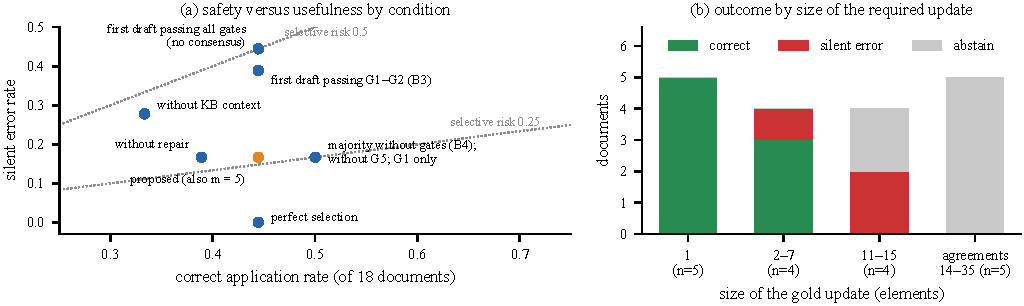
\includegraphics[width=\textwidth]{figs/fig_acquisition.pdf}
\caption{Single-document acquisition on the 18 real documents (13 regulations and 5 collective labor agreements). (a) Silent error rate against correct application rate for each condition; dotted lines mark equal selective risk. (b) Outcome of the pipeline by the number of elements in the gold update.}
\label{fig:acq}
\end{figure*}

Success depended on how much an update had to change (Fig.~\ref{fig:acq}(b)). All five documents whose gold update has one element were applied correctly, and three of the four with 2 to 7 elements. None of the four regulations with 11 to 15 elements was, and neither was any of the five labor agreements with 14 to 35 elements. By change type, 4 of the 5 parameter changes (T1) and 4 of the 8 structural regulations were correct.

The three silent errors are material. Every wrong withholding value differs from the gold value by more than Rp1, and most by more than Rp1,000. The update for E02 (benefits in kind) affected 52 employee-year cases, with a largest withholding difference of Rp61,573,500 and a median relative difference of 19.7\%. The update for E07 (premium relief) affected 42 cases, with a largest difference of Rp279,300, and the update for E11 (government-borne tax for 2026) affected 2 cases, with a largest difference of Rp39,650. Element-level similarity to the gold update did not predict correctness. Five correct updates match their gold update element for element, while the correct update for E03 recovers 3 of 7 gold elements and the correct update for E10 matches none. The wrong updates recover between 13\% and 50\% of the gold elements. Several equivalent updates can state the same regulation, which is why correctness is judged on computed results.

The drafts themselves were often right. The drafts before selection reached pass@1 of 0.667, pass@$m$ of 0.692, and 1@$m$ of 0.615 on the regulations, so consensus did not beat a randomly chosen draft. Of the 49 initial drafts, 17 failed a gate (Table~\ref{tab:gates}) and 11 of those passed after repair. All 18 real documents were judged relevant. Of the 20 distractors, 7 were judged relevant (0.35, CI 0.15--0.59), but only P01 led to a wrong update. Exploratory results complete the picture. The four counterfactual documents gave 1 correct update, 1 wrong update, and 2 abstentions, and no draft reproduced the original value of a counterfactual parameter (0 of 6). The pipeline was correct on 5 of the 14 synthetic policies, wrong on 6, and abstained on 3. Of 28 quotes checked by hand, 23 supported their element and 5 supported it partly.

\subsection{Component Ablation}
\label{sec:res-ablation}
Table~\ref{tab:ablation} isolates the components. Removing the knowledge-base context from the prompt raised the silent errors from 3 to 5 and lowered the correct updates from 8 to 6. Removing G2, G3, or G4 changed no outcome, and keeping only G1 or removing G5 turned one abstention, E04, into a correct update. G5 rejected all three drafts for E04 because their stated effective date, 1 January 2024, changed no generated case in that month. Two of them also carried an element without effect, such as a rule that restated an existing one. Without G5, the consensus of these drafts was correct on the test cases. The three silent errors passed every gate configuration. The reduction of silent errors from 8 for the first passing draft to 3 for the pipeline therefore comes from drawing several drafts and requiring their agreement. The gates did not lower it further on these 18 documents. Perfect selection among the drafts that passed the gates would have removed the three silent errors but added no correct update, so every correct draft that survived the gates was already chosen.

\begin{table}[!t]
\caption{Ablation on the 18 real documents (correct, silent error, abstain). $^{\mathrm{a}}$Amendment. $^{\mathrm{b}}$Recomputed after the main results from the stored drafts, without new model calls.}
\label{tab:ablation}
\centering\footnotesize
\setlength{\tabcolsep}{3pt}
\begin{tabularx}{\columnwidth}{@{}Lccc@{}}
\toprule
Condition & Correct & Silent & Abstain \\
\midrule
Full pipeline & 8 & 3 & 7 \\
Without knowledge-base context$^{\mathrm{a}}$ & 6 & 5 & 7 \\
Without G2$^{\mathrm{b}}$ & 8 & 3 & 7 \\
Without G3$^{\mathrm{b}}$ & 8 & 3 & 7 \\
Without G4 & 8 & 3 & 7 \\
Without G5 & 9 & 3 & 6 \\
G1 only$^{\mathrm{b}}$ & 9 & 3 & 6 \\
Without the repair round & 7 & 3 & 8 \\
Majority vote without gates (B4) & 9 & 3 & 6 \\
First draft passing G1--G2 (B3) & 8 & 7 & 3 \\
First draft passing all gates & 8 & 8 & 2 \\
Perfect selection & 8 & 0 & 10 \\
\bottomrule
\end{tabularx}
\begin{minipage}{\columnwidth}\vspace{2pt}\scriptsize
SHACL in G1 rejected 7 of 319 drafts that had passed the JSON schema. Formalizing a whole legal state from scratch produced no draft that passed the gates, from six drafts on two legal states.
\end{minipage}
\end{table}

\subsection{Chained Replay, 2023--2026}
\label{sec:res-chain}
On the transplanted chain, 31 of 33 events added no new incorrect case (OAR CI 0.798--0.993), which meets H3a (Fig.~\ref{fig:replaychain}). It meets H3a only because new errors appeared at two events, E02 with 15 cases and the distractor P01 with 264 cases. Already 279 of 300 scored cases were wrong after P01, and the count rose to 579 of 600 only because cases of later tax years were added. The high OAR therefore reflects masking, since later events could not add errors to cases that were already wrong.

\begin{figure*}[!t]
\centering
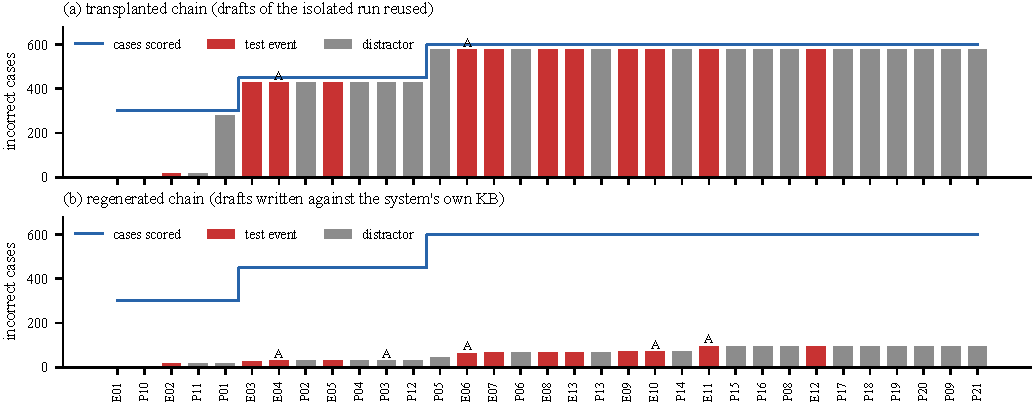
\includegraphics[width=\textwidth]{figs/fig_replay.pdf}
\caption{Regulation replay in chronological order. Bars give the incorrect employee-year cases after each event (red: test event, grey: distractor); the line gives the number of cases scored, which grows as tax years enter; A marks an abstention. Each chain was run once.}
\label{fig:replaychain}
\end{figure*}

The regenerated chain follows Definition~\ref{def:adapt} fully and gives a different picture. Its OAR is 23/33 (CI 0.513--0.844), only 5 of the 13 regulatory events added no new error, and 93 of 600 cases were wrong at the end. Of the 103 new errors, 53 appeared at events where the chain abstained; the abstention on E04 alone added 8. Triggered errors totalled 29 cases on the 13 regulatory events (57 with the distractors), and 26 of them occurred at E10 and E11, where the chain had abstained. Most errors in the chain therefore came from a knowledge base that stayed out of date, not from a wrong update that spread.

\subsection{Cross-Layer Impact Detection}
Of the 134 policy--event pairs, 33 were affected (prevalence 0.25), and 27 of these involved synthetic policies. The frozen detector reached a recall of 0.91 (cluster CI 0.75--1.00), a precision of 0.71, and an $F_2$ of 0.862. Its $F_2$ exceeded that of scanning the policy text without the graph, B5(ii), at 0.669, but not that of flagging every policy that touches $F_\Delta$, B5(i), at 0.868. The three missed pairs involve a policy that produces a fact which changes through an upstream parameter. A second version of the detector, written after these results, closes that gap and becomes identical to B5(i). The execution-based labels and a manual labeling of conflicts agreed poorly (Cohen's $\kappa = -0.018$) because one records a change of value and the other a breach of a rule.

\subsection{Comparison with Code Maintenance and Direct LLM Calculation}
\label{sec:res-compare}
The TER regime consists of 8 new and 13 changed elements of the knowledge base across E03 and E04, with no engine change. Two open-source PPh 21 calculators added TER 26 and 915 days after PP 58/2023 was issued, changing 163 and 504 lines of code (Fig.~\ref{fig:adapt}). The model calls that drafted the two updates took about 12.5 minutes in total, 164 seconds for E03 and 586 seconds for E04. The median over the 18 real documents was about two minutes. Review time was not measured, and the delays of the calculators include development and release practices that this comparison does not control, so the comparison is descriptive. An LLM that computed PPh 21 directly from the case data (B2, exploratory) was exact on 76 of 100 operational cases (CI 0.66--0.84) and within Rp1 on 97. It gave no trace and cost USD 0.068 per case for every computation, whereas the pipeline pays once per document.

\begin{figure}[!t]
\centering
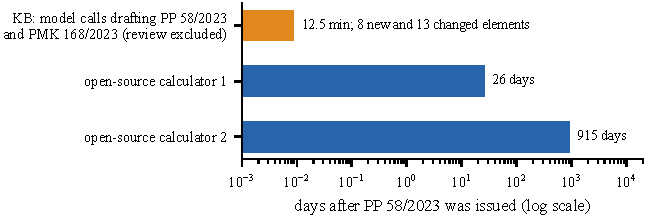
\includegraphics[width=\columnwidth]{figs/fig_adapt.pdf}
\caption{Time to adapt to the TER method after PP 58/2023 was issued: summed duration of the model calls that drafted the knowledge updates (review time not measured) against the commits of two open-source calculators, with the size of each change.}
\label{fig:adapt}
\end{figure}
